\setcounter{Exercise}{4}
\begin{Exercise}
	This problem is quite simple.
	\begin{enumerate}
		\item $4c=5s$ where $c$ is the number of people of ordered cheesecake, and $s$ the number who ordered strudel.
		\item $6s = p$ where $p, s$ is the number of professors and students respectively.
	\end{enumerate}
\end{Exercise}

\begin{Exercise}
Let the height of the crossing be denoted $h$, and let the left pole be of height $x$ and the right pole of height $y$.
We seek to establish a relationship between the three variables, which we will do using similar triangles.

Let the distance between the bases of the two pole be denoted $c = c_1 + c_2$ where $c_1$ is the segment from the left pole
to the crossing, and $c_2$ the segment from the right pole to the crossing. 
We can then write the following expression from viewing the similar triangles:
\begin{align}
	\frac{c_2 x}{c_1 + c_2} = \frac{h}{c_2}
\end{align}
Similarly for the other variable:
\begin{align}
	\frac{c_1 y}{c_1 + c_2} = \frac{h}{c_1}.
\end{align}

Combining the two and solving for $\frac{x}{y}$, we have $\frac{x}{y} = \frac{c_1}{c_2}$. 
Now:
\begin{align}
	h &= \frac{c_2 x}{c_1 + c_2} \\
	&= \frac{x}{\frac{c_1}{c_2} + 1} \\
	&= \frac{x}{\frac{x}{y} + 1} \\
	&= \frac{xy}{x+y}
\end{align} \qed
\end{Exercise}

\begin{Exercise}
	(A bit lazy with the figures for this one, so I'll try to explain this with words).
	Note that there are probably many solutions to this.
	Let $k$ be the length of the right triangle that is opposite angle $\theta$. 
	We can express $k$ as a $\tan(\theta) = \frac{k}{L}$. 

	Since we know the width of the paper, the remaining length is $8-k$. 
	The hypotenuse of the right triangle at the bottom left corner of figure 1.17 is of length $k$ also, as it's simply folded up.
	Only one thing remains, which is that the angle for the right triangle at the bottom is of $2\theta$, by simply tallying up the angles.

	Finally, we have the expression:
	\begin{align}
		\cos(2\theta) = \frac{k}{8-k} \\
		\frac{8\cos(2\theta)}{1 + \cos(2\theta)} &= k \\
		\frac{8\cos(2\theta)}{1 + \cos(2\theta)} &= k \\
		\frac{8\cos(2\theta)}{1 + \cos(2\theta)} &= L\tan(\theta) \\
		L &= \frac{1}{\tan(\theta)}\frac{8\cos(2\theta)}{1 + \cos(2\theta)}
	\end{align}
	One can simplify this more, but the main goal is accomplished.	\qed
\end{Exercise}

\begin{figure}[h]
	\centering
	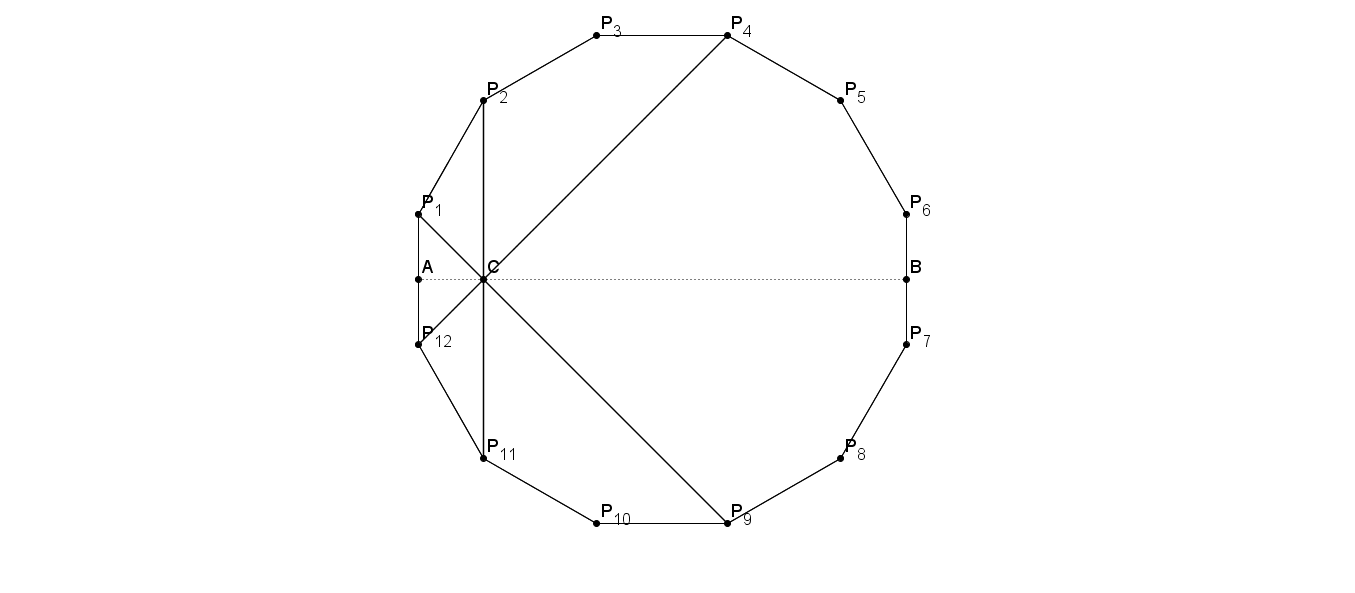
\includegraphics[width=1.2\textwidth]{./figures/chpt1/1_5_8.png}
	\caption{Exercise 1.5.8}
	\label{fig:1_5_8}
\end{figure}

\begin{Exercise}
	We see from figure~\ref{fig:1_5_8} that indeed they are concurrent, but we need to prove this rigorously.

	The angle of $CP_1P_{12} = P_{12}P_1C = 45^{\circ}$ by looking at polygons created by the diagonals itself and the dodecagon.
	If we let the side length of the dodecagon be $x$, then $P_1P_9$ and $P_4P_{12}$ intersects at exactly $x/2$ distance away from the segment $P_1P_{12}$ by the properties of right triangle ($P_1P_{12}C$ is the special right triangle).

	It is obvious that $P_2P_{11}$ creates a trapezoid with angles 150 and 30. 
	Since we have the angle, we can now find the height of the trapezoid, which is exactly $x/2$ as predicted (using $\sin 30^{\circ}$).

	One has to tie this proof a bit tighter for the Putnam exam though by proving the diagonals first intersect line $AB$,
	\footnote{a symmetry argument should do here} but
	this is a good enough sketch I think. \qed
\end{Exercise}

